% \pagebreak[4]
% \hspace*{1cm}
% \pagebreak[4]
% \hspace*{1cm}
% \pagebreak[4]

\chapter{Giới thiệu }
\ifpdf
    \graphicspath{{Chapter1/Chapter1Figs/PNG/}{Chapter1/Chapter1Figs/PDF/}{Chapter1/Chapter1Figs/}}
\else
    \graphicspath{{Chapter1/Chapter1Figs/EPS/}{Chapter1/Chapter1Figs/}}
\fi

Nhờ vào những cải cách trong giao thông và cơ sở hạ tầng viễn thông mà giờ đây toàn cầu hóa đang trở nên gần với chúng ta hơn bao giờ hết. Trong xu hướng đó nhu cầu giao tiếp và thông hiểu giữa những nền văn hóa là không thể thiếu. Tuy nhiên, những nền văn hóa khác nhau thường kèm theo đó là sự khác biệt về ngôn ngữ, là một trong những trở ngại lớn nhất của sự giao tiếp. Một người phải mất rất nhiều thời gian để thành thạo một ngôn ngữ không phải là tiếng mẹ đẻ, và không thể nào học được nhiều ngôn ngữ cùng lúc. Cho nên, việc phát triển một công cụ để giải quyết vấn đề này là tất yếu. Một trong những công cụ như vậy là \textit{Dịch máy}.

\textit{Dịch máy} là quá trình chuyển đổi văn bản/tiếng nói từ ngôn ngữ này sang dạng tương ứng của nó trong một ngôn ngữ khác, được thực hiện bởi một chương trình máy tính nhằm mục đích cung cấp bản dịch tốt nhất mà không cần sự trợ giúp của con người.

Dịch máy có một quá trình lịch sử lâu dài. Từ thế kỷ XVII, đã có những ý tưởng về việc cơ giới hóa quá trình dịch thuật. Tuy nhiên, đến thế kỷ XX, những nghiên cứu về dịch máy mới thật sự bắt đầu. Vào những năm 1930, Georges Artsrouni người Pháp và Petr Troyanskii người Nga đã nộp bằng sáng chế cho công trình có tên "máy dịch" của riêng họ. Trong số hai người, công trình của Troyanskii có ý nghĩa hơn. Nó đề xuất không chỉ một phương pháp cho bộ từ điển tự động, mà còn là lược đồ cho việc mã hóa các vai trò ngữ pháp song ngữ và một phác thảo về cách phân tích và tổng hợp có thể hoạt động. Tuy nhiên, những ý tưởng của Troyanskii đã không được biết đến cho đến cuối những năm 1950. Trước đó, máy tính đã được phát minh.

Những nỗ lực xây dựng hệ thống dịch máy bắt đầu ngay sau khi máy tính ra đời. Có thể nói, chiến tranh và sự thù địch giữa các quốc gia là động lực lớn nhất cho dịch máy thời bấy giờ. Trong Thế chiến thứ II, máy tính đã được quân đội Anh sử dụng trong việc giải mã các thông điệp được mã hóa của quân Đức. Việc làm này có thể coi là một dạng ẩn dụ của dịch máy khi người ta cố gắng dịch từ tiếng Đức được mã hóa sang tiếng Anh. Trong thời kỳ chiến tranh lạnh, vào tháng 7/1949, Warren Weaver, người được xem là nhà tiên phong trong lĩnh vực dịch máy, đã viết một bản ghi nhớ đưa ra các đề xuất khác nhau của ông trong lĩnh vực này. Những đề xuất đó dựa trên thành công của máy phá mã, sự phát triển của lý thuyết thông tin bởi Claude Shannon và suy đoán về các nguyên tắc phổ quát cơ bản của ngôn ngữ. Trong vòng một năm, một vài nghiên cứu về dịch máy đã bắt đầu tại nhiều trường đại học của Mỹ. Vào ngày 7/1/1954, tại trụ sở chính của IBM ở New York, thử nghiệm Georgetown-IBM được tiến hành. Máy tính IBM 701 đã tự động dịch 49 câu tiếng Nga sang tiếng Anh lần đầu tiên trong lịch sử chỉ sử dụng 250 từ vựng và sáu luật ngữ pháp \cite{hutchins}. Thí nghiệm này được xem như là một thành công và mở ra kỉ nguyên cho những nghiên cứu với kinh phí lớn về dịch máy ở Hoa Kỳ. Ở Liên Xô những thí nghiệm tương tự cũng được thực hiện không lâu sau đó.

%Dịch máy có một quá trình lịch sử lâu dài, từ thế kỷ 17, đã có những ý tưởng về một loại ngôn ngữ mang ý nghĩa phổ quát nhưng mãi đến những năm 1950 những nghiên cứu về dịch máy mới thật sự bắt đầu \cite{hutchins}. Trong thời kì Chiến tranh Lạnh, vào ngày 7 tháng 1 năm 1954, tại trụ sở chính của IBM ở New York, thử nghiệm Georgetown-IBM được tiến hành. Máy tính IBM 701 đã tự động dịch 49 câu tiếng Nga sang tiếng Anh lần đầu tiên trong lịch sử chỉ sử dụng 250 từ vựng và sáu luật ngữ pháp \cite{hutchins}. Thí nghiệm này được xem như là một thành công và mở ra kỉ nguyên cho những nghiên cứu với kinh phí lớn về dịch máy ở Hoa Kỳ. Ở Liên Xô những thí nghiệm tương tự cũng được thực hiện không lâu sau đó.

Trong một thập kỷ tiếp theo, nhiều nhóm nghiên cứu về dịch máy được thành lập. Một số nhóm chấp nhận phương pháp thử và sai, thường dựa trên thống kê với mục tiêu là một hệ thống dịch máy có thể hoạt động ngay lập tức, tiêu biểu như: nhóm nghiên cứu tại đại học Washington (và sau này là IBM) với hệ thống dịch Nga-Anh cho Không quân Hoa Kỳ, những nghiên cứu tại viện Cơ học Chính xác ở Liên Xô và Phòng thí nghiệm Vật lý Quốc gia ở Anh. Trong khi một số khác hướng đến giải pháp lâu dài với hướng tiếp cận lý thuyết bao gồm cả những vấn đề liên quan đến ngôn ngữ cơ bản như nhóm nghiên cứu tại Trung tâm nghiên cứu lý thuyết tại MIT, Đại học Havard và Đơn vị nghiên cứu ngôn ngữ Đại học Cambridge. Những nghiên cứu trong giai đoạn này có tầm quan trọng và ảnh hưởng lâu dài không chỉ cho Dịch máy mà còn cho nhiều ngành khác như Ngôn ngữ học tính toán, Trí tuệ nhân tạo - cụ thể là việc phát triển các từ điển tự động và kỹ thuật phân tích cú pháp. Nhiều nhóm nghiên cứu đã đóng góp đáng kể cho việc phát triển lý thuyết ngôn ngữ. Tuy nhiên, mục tiêu cơ bản của dịch máy là xây dựng hệ thống có khả năng tạo ra bản dịch tốt lại không đạt được dẫn đến một kết quả là vào năm 1966 bản báo cáo từ Ủy ban tư vấn xử lý ngôn ngữ tự động (Automatic Language Processing Advisory) của Hoa Kỳ, tuyên bố rằng dịch máy là đắt tiền, không chính xác và không mang lại kết quả hứa hẹn \cite{hutchins}. Thay vào đó, họ đề nghị tập trung vào phát triển các từ điển, điều này đã loại bỏ các nhà nghiên cứu Mỹ ra khỏi cuộc đua trong gần một thập kỷ.

%Từ đó đến nay, đã có nhiều hướng tiếp cập đã được sử dụng trong dịch máy với mục tiêu tạo ra bản dịch có độ chính xác cao và giảm thiểu công sức của con người đặc biệt phải kể đến Dịch máy dựa trên luật, Dịch máy thống kê hay gần đây nhất là Dịch máy Nơ-ron (hình 1.1).

\begin{figure}
	\centering
	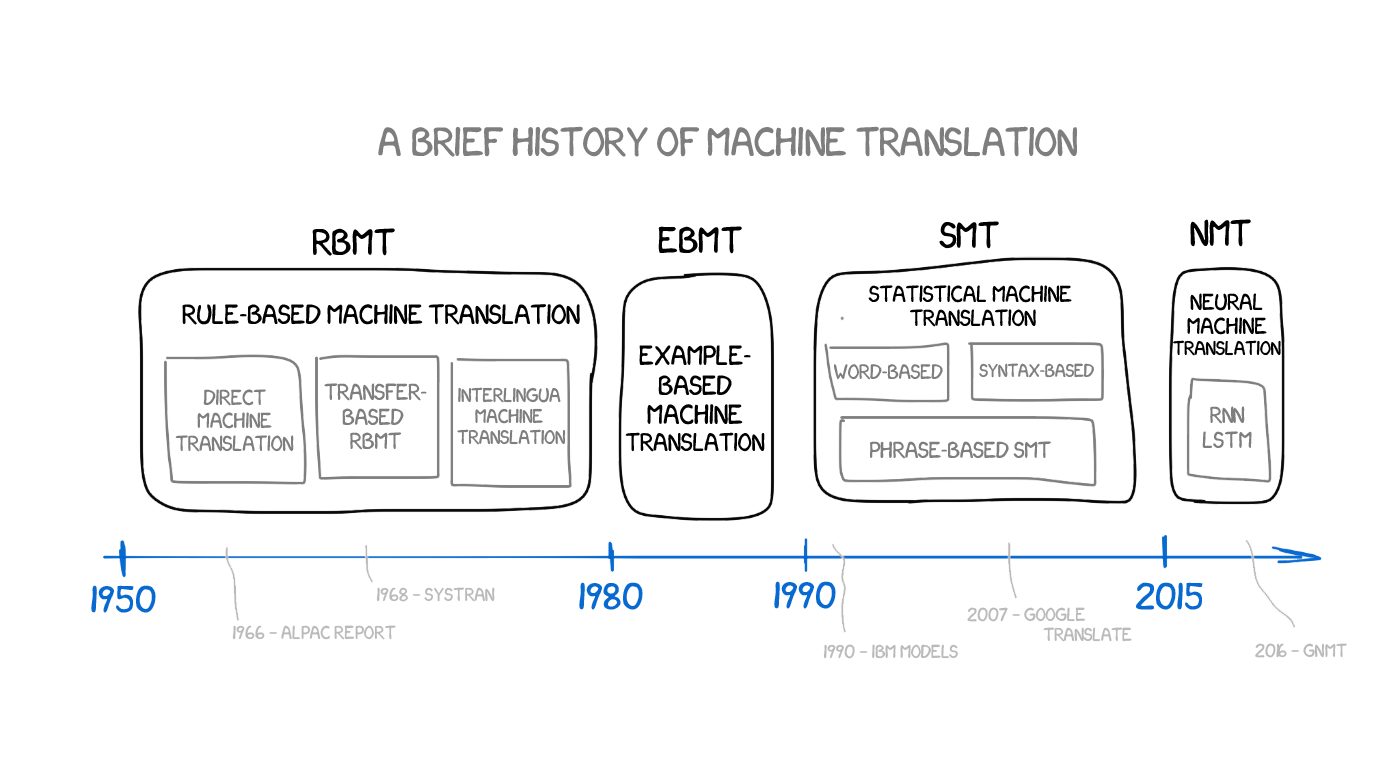
\includegraphics[width=\textwidth]{mthistory}
	\caption[Lịch sử tóm tắt của dịch máy]{Lịch sử tóm tắt của dịch máy, nguồn ảnh: Ilya Pestov trong blog \href{https://medium.freecodecamp.org/a-history-of-machine-translation-from-the-cold-war-to-deep-learning-f1d335ce8b5}{A history of machine translation from the Cold War to deep learning}}
	\label{fig_mthistory}
\end{figure}

%Trong những năm tiếp theo, Dịch máy đã trải qua nhiều giai đoạn phát triển lớn nhưng cũng gặp phải một số trì trệ, đáng kể nhất là vào năm 1966 bản báo cáo từ ủy ban ALPAC (Automatic Language Processing Advisory) của Hoa Kỳ, tuyên bố rằng Dịch máy là đắt tiền, không chính xác và không mang lại kết quả hứa hẹn. Thay vào đó, họ đề nghị tập trung vào phát triển các từ điển, điều này đã loại bỏ các nhà nghiên cứu Mỹ ra khỏi cuộc đua trong gần một thập kỷ.

%Mặc dù vậy, cơ sở cho việc Xử lý ngôn ngữ tự nhiên hiện đại đã được tạo ra chỉ bởi các nhà khoa học và nỗ lực, nghiên cứu và phát triển của họ. 

\section{Các phương pháp Dịch máy}
Từ đó đến nay, đã có nhiều hướng tiếp cập đã được sử dụng trong dịch máy với mục tiêu tạo ra bản dịch có độ chính xác cao và giảm thiểu công sức của con người. Trong những năm đầu tiên, để tạo ra bản dịch tốt, các phương pháp thời bấy giờ đều hỏi hỏi những lý thuyết tinh vi về ngôn ngữ học. 


Từ đó đến nay, đã có nhiều hướng tiếp cập đã được sử dụng trong dịch máy với mục tiêu tạo ra bản dịch có độ chính xác cao và giảm thiểu công sức của con người có thể chia làm hai nhóm. Nhóm đầu tiên là những hướng tiếp cận dựa trên \textit{Từ điển} (Dictionary based). Đây là hướng tiếp cận chính cho những nghiên cứu về dịch máy trong những năm 1950-1960. Những phương pháp dựa trên hướng tiếp cập từ điển có thể kể đến như \textit{Dịch máy trực tiếp} (Direct machine translation), \textit{Dịch máy chuyển dịch} (Transfer-based machine translation) hay \textit{Dịch máy ngôn ngữ đại diện} (Interlingual machine translation). Điểm chung của những phương pháp này là dùng một từ điển để dịch các từ từ ngôn ngữ nguồn sang ngôn ngữ đích và sau đó cố gắng chỉnh sửa bản dịch để tạo ra một câu có nghĩa. Nhóm phương pháp này thường yêu cầu một bộ từ điển giữa hai ngôn ngữ cần dịch và một tập các quy tắc ngữ pháp cho mỗi ngôn ngữ. Bản dịch của hướng tiếp cận Từ điển thường có chất lượng kém và không sử dụng được trừ một số trường hợp đặc biệt. Ngoài ra chúng còn đòi hỏi một lượng nhân lực lớn với hiểu biết sâu sắc cho việc xây dựng những bộ từ điển và các quy tắc ngôn ngữ. 

Nhóm thứ hai là những hướng tiếp cận dựa trên \textit{Ngữ liệu} (Corpus based). Nhóm này hoạt động dựa trên một tập dữ liệu song song của các cặp câu là bản dịch của nhau trong hai ngôn ngữ gọi là ngữ liệu và chỉ yêu cầu những tri thức tối thiểu về ngôn ngữ học. Trước khi dịch máy nơ-ron ra đời, phương pháp nổi bật và hiệu quả nhất dựa trên hướng tiếp cận này chính là \textit{Dịch máy thống kê} (Statistical machine translation). Vào năm 1990, IBM công bố hệ thống dịch máy thống kê của họ, đây là hệ thống đầu tiên có khả năng tạo ra bản dịch mà không cần biết gì về các từ hay quy tắc ngữ pháp của ngôn ngữ. Chỉ cần cung cấp bộ ngữ liệu, hệ thống này phân tích các câu tương ứng trong ngữ liệu đó để hiểu được các mô hình bên dưới.

\begin{figure}
	\centering
	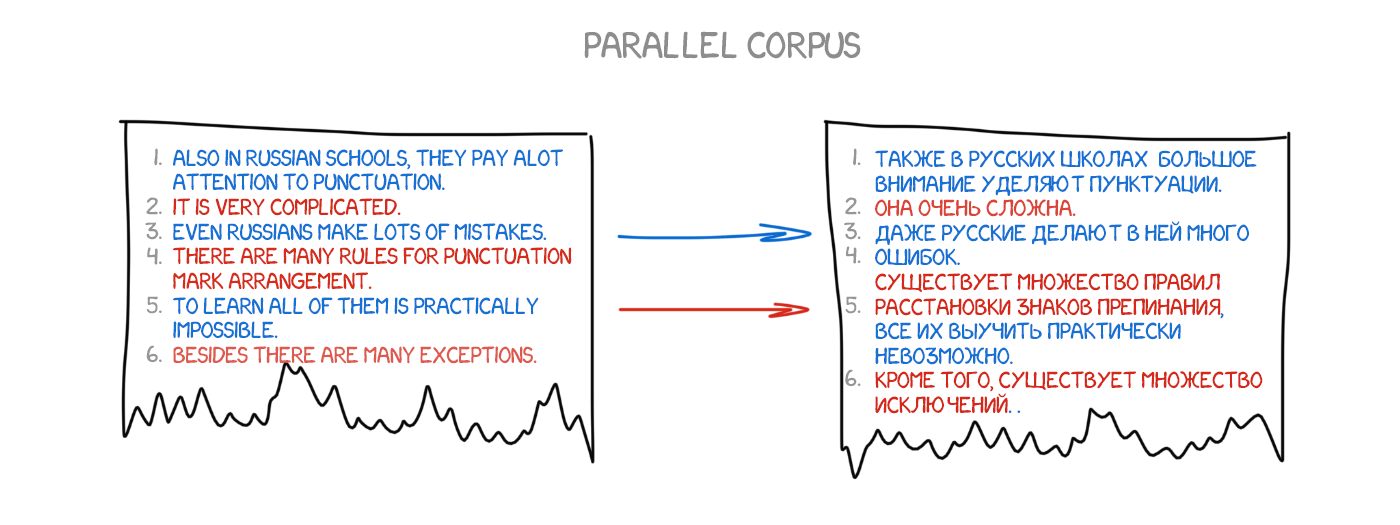
\includegraphics[width=\textwidth]{smt}
	\caption[Ví dụ về tập các câu song song trong hai ngôn ngữ]{Ví dụ về tập các câu song song trong hai ngôn ngữ}
	\label{fig_parallelcorpus}
\end{figure}


\section{Dịch máy Nơ-ron}

Mặc dù trên thực tế đã có nhiều hệ thống dịch máy được phát triển dựa trên dịch máy thống kê thời bấy giờ, tuy nhiên nó không hoạt động thực sự tốt bởi một số nguyên nhân. Một là việc những từ hay đoạn được dịch cục bộ và quan hệ của chúng với những từ cách xa trong câu nguồn thường bị bỏ qua. Hai là mô hình ngôn ngữ N-gram hoạt động không thực sự tốt đối với những bản dịch dài và ta phải tốn nhiều bộ nhớ để lưu trữ chúng. Ngoài ra việc sử dụng nhiều thành phần nhỏ được điều chỉnh riêng biệt như mô hình dịch, mô hình ngôn ngữ, gióng hàng,.. cũng gây khó khăn cho việc vận hành và phát triển mô hình này.

% TODO: Kalchbrenner and Blunsom (2013), Sutskever et al. (2014) and Cho et al. (2014b)
\textit{Dịch máy nơ-ron} (Neural machine translation) là một hướng tiếp cận mới trong dịch máy trong những năm gần đây được đề xuất đầu tiên bởi \cite{kalchbrennerBlunsom}, \cite{sutskever}, \cite{cho}. Giống như dịch máy thống kê, dịch máy nơ-ron cũng là một phương pháp thuộc hướng tiếp cận dựa trên ngữ liệu, trong khi dịch máy thống kê bao gồm nhiều mô-đun nhỏ được điều chỉnh riêng biệt, Dịch máy nơ-ron cố gắng dùng một mạng nơ-ron như là thành phần duy nhất của hệ thống, mọi thiết lập sẽ được thực hiện trên mạng này. 

% TODO: Sutskever et al., 2014; Cho et al., 2014a
Hầu hết những mô hình dịch máy nơ-ron đều dựa trên kiến trúc \textit{Bộ mã hóa - Bộ giải mã} (Encoder-Decoder) (\cite{sutskever}, \cite{cho}). Bộ mã hóa thường là một mạng nơ-ron có tác dụng \textit{"nén"} tất cả thông tin của câu trong ngôn ngữ nguồn vào một vector có kích thước cố định. Bộ giải mã, cũng là một mạng nơ-ron, sẽ tạo bản dịch trong ngôn ngữ đích từ vector có kích thước cố định kia. Toàn bộ hệ thống bao gồm bộ mã hóa và bộ giải mã sẽ được huấn luyện \textit{"end-to-end"} để tạo ra bản dịch, quá trình này được mô tả như hình 1.2.

\begin{figure}
	\centering
	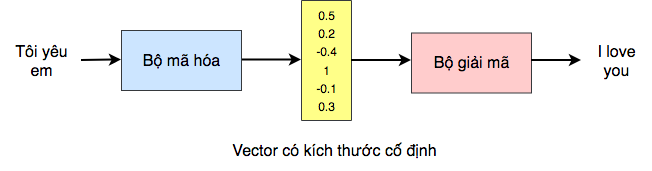
\includegraphics[width=\textwidth]{intro2nmt}
	\caption[Ví dụ về Kiến trúc \textit{bộ mã hóa - bộ giải mã} trong dịch máy nơ-ron]{Ví dụ về kiến trúc bộ mã hóa - bộ giải mã trong dịch máy nơ-ron}
	\label{fig_encoder_decoder}
\end{figure}

% TODO: mention LSTM
Trong thực tế cả bộ mã hóa và giải mã thường dựa trên một mô hình mạng nơ-ron tên là \textit{Mạng nơ-ron hồi quy} là một thiết kế mạng đặc trưng cho việc xử lý dữ liệu chuỗi. Mạng nơ-ron hồi quy cho phép chúng ta mô hình hóa những dữ liệu có độ dài không xác định, rất thích hợp cho bài toán dịch máy. Hình 1.3 mô tả chi tiết hơn về kiến trúc bộ mã hóa - giải mã sử dụng mạng nơ-ron hồi quy. Đầu tiên bộ mã hóa đọc qua toàn bộ câu nguồn và tạo ra một vector đại diện gọi là \textit{vector trạng thái}. Điều này giúp cho toàn bộ những thông tin cần thiết hay quan hệ giữa các từ đều được tập hợp vào một nơi duy nhất. Bộ giải mã, lúc này đóng vai trò như một mô hình ngôn ngữ để tạo ra từng từ trong ngôn ngữ đích và sẽ dừng lại đến khi một ký tự đặc biệt xuất hiện.

\begin{figure}
	\centering
	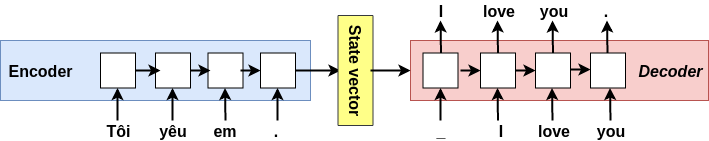
\includegraphics[width=\textwidth]{encoder-decoder}
	\caption[Kiến trúc bộ mã hóa - bộ giải mã được xây dựng trên mạng nơ-ron hồi quy]{Kiến trúc bộ mã hóa - bộ giải mã được xây dựng trên mạng nơ-ron hồi quy}
	\label{fig_encoder_decoder_details}
\end{figure}

Trong hình 2, có thể thấy rằng bộ giải mã tạo ra bản dịch chỉ dựa trên trạng thái ẩn cuối cùng, cũng chính là vector có kích thước cố định được tạo ra ở bộ mã hóa. Vector này phải mã hóa mọi thứ chúng ta cần biết về câu nguồn. Giả sử chúng ta có câu nguồn với độ dài là 50 từ, từ đầu tiên ở câu đích có lẽ sẽ có mối tương quan cao với từ đầu tiên ở câu nguồn. Điều này có nghĩa là bộ giải mã phải xem xét thông tin được mã hóa từ 50 \textit{"time step"} trước đó. Mạng nơ-ron hồi quy được chứng minh là gặp khó khăn trong việc mã hóa những chuỗi dài \cite{difficultyRNN}. Để giải quyết vấn đề này, thay vì dùng mạng nơ-ron hồi quy thuần, người ta sử dụng các biến thể của nó quy như \textit{Long short-term memory (LSTM)}. Trên lý thuyết, LSTM có thể giải quyết vấn đề mất mát thông tin trong chuỗi dài, nhưng trong thực tế vấn đề này vẫn chưa thể được giải quyết hoàn toàn. Một số nhà nghiên cứu đã phát hiện ra rằng đảo ngược chuỗi nguồn trước khi đưa vào bộ mã hóa tạo ra kết quả tốt hơn một cách đáng kể \cite{sutskever} bởi nó khiến cho những từ đầu tiên được đưa vào bộ mã hóa sau cùng, và được giải mã thành từ tương ứng ngay sau đó. Cách làm này tuy giúp cho bản dịch hoạt động tốt hơn trong thực tế, nhưng nó không phải là một giải pháp về mặt thuật toán. Hầu hết các đánh giá về dịch máy được thực hiện trên các ngôn ngữ như ngôn ngữ có trật tự câu tương đối giống nhau. Ví dụ trật tự dạng "chủ ngữ - động từ - vị ngữ" như tiếng Anh, Đức, Pháp hay Trung Quốc. Đối với dạng ngôn ngữ có một trật tự khác ví dụ "chủ ngữ - vị ngữ - động từ" như tiếng Nhật, đảo ngược câu nguồn sẽ không hiệu quả.

\textit{Attention} là cơ chế giải phóng kiến trúc bộ mã hóa - bộ giải mã khỏi nhược điểm chỉ sử dụng một vector có chiều dài cố định làm đại diện cho câu đầu vào. Ý tưởng chính của cơ chế này là ở mỗi thời điểm phát sinh các từ trong bản dịch, bộ giải mã sẽ "nhìn" vào các phần khác nhau của câu nguồn trong quá trình mã hóa. Quan trọng hơn, cơ chế này cho phép mô hình học được cách chọn những phần cần thiết để tập trung vào dựa trên câu nguồn và những gì mà bộ giải mã đã giải mã được.

\begin{figure}
	\centering
	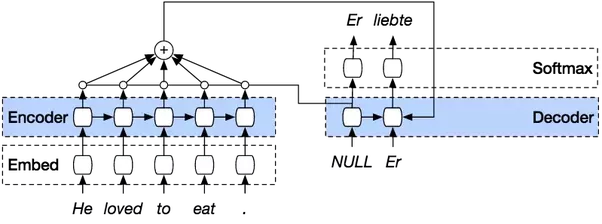
\includegraphics[width=\textwidth]{intro2attention}
	\caption[Cơ chế Attention trong dịch máy nơ-ron]{Cơ chế Attention trong dịch máy nơ-ron}
	\label{fig_introattention}
\end{figure} 

\section{Cấu trúc của khóa luận}
Trong khóa luận này, chúng tôi quyết định tập trung nghiên cứu về dịch máy nơ-ron và cơ chế Attention dựa trên nghiên cứu của nhóm tác giả tại đại học Stanford bao gồm Minh-Thang Luong, Hieu Pham, Christopher Manning trong bài báo \textit{Effective Approaches to Attention-based Neural Machine Translation} \cite{mainpaper}. Các phần còn lại trong luận văn được trình bày như sau:

\begin{itemize}
	\item[•] Chương 2 trình bày về những thành nền tảng của kiến trúc bộ mã hóa - giải mã
	
	\item[•] Chương 3 trình bày về cơ chế Attention, đây là phần chính của luận văn. Trong phần này gồm có hai phần nhỏ:
		\begin{itemize}
			\item[-] \textit{Global attetion}: là cơ chế tập trung vào tất cả các trạng thái ở câu nguồn
			\item[-] \textit{Local attetion}: tập trung vào một tập các trạng thái ở câu nguồn tại một thời điểm
		\end{itemize}
	\item[•] Chương 4 trình bày về các thí nghiệm và các phân tích về kết quả đạt trên hai tập dữ liệu Anh-Đức, Anh-Việt.
	\item[•] Kết luận và hướng phát triển của luận văn.
\end{itemize}





